\documentclass[11pt,letterpaper]{article}
\usepackage[margin=1in]{geometry}
\usepackage{amsmath,amssymb,amsthm,booktabs,graphicx,xcolor}
\usepackage[hidelinks]{hyperref}
\usepackage{microtype}
\definecolor{navy}{HTML}{173754}
\hypersetup{colorlinks=true,linkcolor=navy,citecolor=navy,urlcolor=navy,
  pdftitle={Stability and Information Sensitivity in Transformer In-Context Inverse Learning}}
\newtheorem{theorem}{Theorem}
\DeclareMathOperator{\diag}{diag}
\DeclareMathOperator{\softmax}{softmax}
\newcommand{\norm}[1]{\lVert #1\rVert_2}
\newcommand{\tf}{f_\phi}
\newcommand{\pct}[1]{#1\%}
\setlength{\emergencystretch}{2em}
\title{\textbf{Stability and Information Sensitivity in\\Transformer In-Context Inverse Learning}}
\author{CS 886 Course Project}
\date{November 2026}

\begin{document}
\maketitle

\begin{abstract}
How do Transformers balance low replacement sensitivity with the ability
to learn from a highly informative observation? We study a frozen,
mean-pooled Transformer that estimates latent generator costs from
economic-dispatch records. For the implemented architecture, a single
bounded-record replacement changes the parameter estimate by at most
\(C/m\), where \(m\) is context length. We construct two valid,
individually identifying dispatch contexts whose costs remain a fixed
distance apart even though their records differ at only one price.
This gives a worst-case recovery error floor for any estimator with a
\(C/m\) sensitivity guarantee. Across three training seeds, matched
price perturbations elicit a \(14.1\times\) larger Transformer response
at high versus low leverage. On the identifying pair at \(m=64\),
the model recovers \pct{47.4} of the true parameter difference along
its direction, versus \pct{99.9} for ridge. These results connect the
architecture's stability with the information available in a context.
\end{abstract}

\section{Introduction}
An in-context learner can adapt its output to examples without updating
its weights. Li et al.\ relate its generalization to the stability of the
algorithm implemented by the Transformer \cite{li}. In an inverse
problem, a record can contain information that the rest of the context
lacks. A learner that responds only weakly to every single-record
replacement can then struggle to recover the task that generated the
records. The question is particularly clear when two tasks agree on
an arbitrarily long shared context and differ on one decisive record.

We use inverse economic dispatch because optimal outputs and clearing
prices constrain generator costs through known optimality conditions.
This allows us to distinguish local statistical leverage, the
conditioning of all observations together, and partial identification
on the same physical model. We analyze an upper bound for the actual
encoder and a complementary lower bound from a valid pair of contexts.
We then compare measured response and recovery across architectures,
source-task budgets, and changes to the information in a context.

\clearpage
\section{Problem setup and architecture}
\paragraph{Forward and inverse problems.}
At demand \(d\in[0,2]\), two generators with unit capacity dispatch
according to
\begin{equation}
 \min_{x_1+x_2=d,\ 0\le x_i\le 1}
 \sum_{i=1}^{2}\left(a_i x_i+\tfrac12 b_i x_i^2\right).
 \label{eq:dispatch}
\end{equation}
Each task has one cost vector
\(\theta=(a_1,b_1,a_2,b_2)\) with \(a_i\in[1,1.65]\) and
\(b_i\in[0.8,2]\). Positive quadratic coefficients make the optimal
dispatch unique. For each solve we observe demand, dispatch, the
clearing price \(\lambda\), and each generator's bound status. We use
the sign convention in which a price equals the marginal cost of an
interior generator. For generator \(i\) the KKT conditions give
\begin{equation}
a_i+b_ix_i-\lambda
\begin{cases}
=0 & \text{if }0<x_i<1,\\
\geq 0 & \text{if }x_i=0,\\
\leq 0 & \text{if }x_i=1 .
\end{cases}
\label{eq:kkt}
\end{equation}
The inverse problem estimates \(\theta\) from \(m\) such records from one
task. Marginal costs are inferred from optimal decisions and prices,
as in related inverse optimization methods \cite{keshavarz,liang}.
Here the feasible set and synthetic optimality conditions also let us
design specific test interventions.

\paragraph{Information in the context.}
For \(u_{it}=(1,x_{it})^\top\) let
\(H_i=m^{-1}\sum_{t:\,0<x_{it}<1}u_{it}u_{it}^{\top}\).
Two distinct interior outputs give two independent equations for a
generator. In contrast, repeated or tightly clustered outputs leave a
direction unconstrained or weakly conditioned. We use
\(\min_i\lambda_{\min}(H_i)\) as the context's information
diagnostic and the diameter of the set of box-constrained costs
satisfying \eqref{eq:kkt} as an ambiguity diagnostic. Bound records
can shrink this admissible set through inequalities.

\paragraph{Frozen set encoder.}
Each record has four scaled real features
\((d/2,x_1,x_2,\lambda/3.65)\) and six one-hot status features.
An affine embedding of width 64 feeds two unmasked full-attention
encoder layers with four heads, post-residual LayerNorm,
and a width-128 ReLU feedforward block. There are no positional
embeddings and dropout is zero. Mean pooling, an affine readout,
sigmoid, and rescaling to the cost box yield \(\tf(S)\in\mathbb R^4\).
Training minimizes span-normalized squared parameter error over source
tasks. The parameters \(\phi\) stay fixed at evaluation.

This setup is \emph{context-conditioned, supervised amortized inverse
estimation}. The prediction is a parameter vector for the whole task.
In Li et al., the input includes a query and the model predicts its
response from a sequence of example pairs \cite{li}. Comparisons with
ridge are motivated by prior work on learned linear-model algorithms
in query-conditioned ICL \cite{akyurek}. Our inputs and output metric
test a related inverse estimation problem.

\clearpage
\section{Theoretical analysis}
\begin{theorem}[Replacement stability of the set encoder]
\label{thm:upper}
Fix the finite weights and depth of the architecture above, with positive
LayerNorm epsilon. On any uniformly bounded record domain, there is a
finite \(C\) independent of \(m\) such that, in exact arithmetic,
\(\norm{\tf(S)-\tf(S')} \le C/m\) whenever \(S,S'\) have length \(m\)
and differ at one position.
\end{theorem}

The proof in Appendix~\ref{app:encoder} controls the average state
difference over rows. For bounded scores, each attention probability is
\(O(1/m)\), and the softmax differential bounds the effects of both
changing a query and changing the keys. A fixed-depth composition
preserves the rate through residuals, LayerNorm and the feedforward
blocks. Mean pooling converts the final average row difference into a
prediction bound. Li et al.'s Theorem 3.2 instead controls a designated
query-token output under their normalization assumptions \cite{li}.
Here the constant depends on trained weights and may be large.
The theorem makes a worst-case statement over bounded inputs.

\begin{theorem}[Necessary response for accurate recovery]
\label{thm:lower}
Let two length-\(m\) contexts \(S,S'\) differ in one record, with true
parameters \(\theta,\theta'\) separated by \(D=\norm{\theta-\theta'}\).
If an estimator \(f\) has Euclidean error at most \(\epsilon\) at each
context, then \(\norm{f(S)-f(S')}\ge D-2\epsilon\). If its
replacement sensitivity is at most \(C/m\) on this pair, then
\(\epsilon\ge \tfrac12(D-C/m)_+\).
\end{theorem}
\begin{proof}
Decompose \(\theta-\theta'=(\theta-f(S))+(f(S)-f(S'))+
(f(S')-\theta')\). By the triangle inequality the norm of the middle
term is at least \(D-\norm{f(S)-\theta}-\norm{f(S')-\theta'}\).
Substituting the assumed errors and the optional upper bound gives
the two claims.
\end{proof}

\paragraph{A valid dispatch pair.}
Use \((a_i,b_i)=(1.6,1.0)\) in task A and \((1.2,1.8)\) in task B,
for both generators. Symmetry and strict convexity in
\eqref{eq:dispatch} give \(x_i=d/2\). At \(d=1\), the two tasks give
the same price \(2.1\). At \(d=1.6\), the price is \(2.40\) in A
and \(2.64\) in B. Both demands have interior dispatch. The two
observed prices at outputs \(0.5\) and \(0.8\) uniquely identify each
unit's affine marginal cost. Repeat the common record \(m-1\) times
and place the identifying record last. The pair differs only at that
price, with \(D=\sqrt{1.6}\) independent of \(m\).

Theorem~\ref{thm:lower} is a deterministic statement about any estimator,
related to prior work on stability-constrained estimation \cite{clb}.
Theorems~\ref{thm:upper} and \ref{thm:lower} together imply a
nonvanishing worst-case error floor over this family as \(m\) increases
for a fixed encoder. The repeated-demand construction is a stress case.
In ordinary same-task replacements, the true cost vector stays fixed.
A supporting task-level transfer bound is given in Appendix~\ref{app:transfer}.

\clearpage
\section{Experimental setup}
All reported estimates are taken directly from each learner. The main
studies use seeds 886, 1729, and 2027, with disjoint source, validation,
and test tasks. Each seed has 96 validation and 128 test tasks.
Except when the context is deliberately constructed, demands are drawn
uniformly from \([0,2]\). The architecture and leverage studies use
1,536 source tasks. The architecture comparison uses the same training
protocol across models, with AdamW, batch size 32 and 14 training
epochs. The checkpoint is selected on validation tasks. The
norm-controlled model caps the spectral norm of each attention
Q, K, V and output projection at 0.85. The DeepSets comparator learns
rowwise features and averages them before its readout \cite{deepsets}.

We use relative parameter error
\(\norm{f(S)-\theta}/\norm{\theta}\) for ordinary recovery, Euclidean
error for the deterministic tradeoff, and
\(\norm{f(S)-f(S')}\) for observed replacement sensitivity.
Reported averages weight seeds equally. Where shown, uncertainty is
the standard deviation across seed means. A mean over replacements
estimates a protocol-dependent sensitivity, whereas Theorem~\ref{thm:upper}
applies uniformly to any eligible replacement.

\section{Results}
\subsection{Architecture and same-task stability (D)}
For each unseen task and \(m\in\{4,8,16,32,64\}\), D replaces one
record with a new valid record from that same task, with four trials
per task. The original Transformer achieved the lowest mean
sensitivity and recovery error at every length among the three direct
learners in Table~\ref{tab:d}. The gap narrows in absolute sensitivity as
contexts grow. A function can be very stable by ignoring a direction
needed for identification, so the recovery errors help interpret this
comparison.

\begin{table}[ht]
\centering
\small
\begin{tabular}{r rrr rrr}
\toprule
&\multicolumn{3}{c}{Mean Euclidean prediction change}
&\multicolumn{3}{c}{Relative recovery error (\%)}\\
\cmidrule(lr){2-4}\cmidrule(lr){5-7}
\(m\)&Transformer&Norm cap&DeepSets&Transformer&Norm cap&DeepSets\\
\midrule
4  &0.07750&0.11445&0.11455&5.20&7.03&13.06\\
8  &0.02852&0.05117&0.06152&3.50&5.31&11.75\\
16 &0.01077&0.02273&0.02909&2.92&4.53&11.11\\
32 &0.00461&0.01062&0.01542&2.71&4.14&10.60\\
64 &0.00213&0.00510&0.00760&2.65&3.95&10.28\\
\bottomrule
\end{tabular}
\caption{Single-record replacement within a fixed task and parameter
recovery on the original context. Cells are means over three seeds.}
\label{tab:d}
\end{table}

One explanation consistent with these results is that learned attention
combines records to estimate the shared cost parameters, while the
tight cap restricts that flexibility. An operator cap controls only
part of the architecture bound. Training also changes the other
operators, and the observed averages depend on which records are
replaced. The comparison supports an empirical ordering under this
training and evaluation protocol.

\clearpage
\subsection{Transfer across source-task budgets (E)}
The equal-pass sweep holds the number of passes over each source set
fixed at 14, whereas the equal-step sweep gives every model 448
optimizer updates. Table~\ref{tab:e} shows performance on unseen
target tasks. Under equal passes, task count and optimizer updates
increase together. Under equal steps, the target error stays between
\pct{3.20} and \pct{3.56} and has no monotone trend. Fresh source
contexts estimate source-task risk, while separate unseen targets
estimate transfer risk. For example, the equal-step runs at
\(T=128\) and \(T=1536\) have mean span-scaled target risks
0.002686 and 0.003218, and target-minus-source gaps 0.000517 and
0.000006, respectively. The smaller gap coexists with a higher
absolute target risk. In a separate fixed-length control with
384 updates and 196,608 training records, target errors at \(m=32\)
were \pct{3.48}, \pct{3.25}, and \pct{3.54} for \(T=128,512,1536\).
These controls leave the benefit of task count alone unresolved.

\begin{table}[ht]
\centering
\small
\begin{tabular}{r rr r}
\toprule
&\multicolumn{2}{c}{Equal passes}&Equal steps\\
\cmidrule(lr){2-3}
Source tasks \(T\)&Updates&Target error (\%)&Target error (\%)\\
\midrule
128   &56  &13.48&3.29\\
256   &112 &10.45&3.47\\
512   &224 &7.46&3.54\\
1,024 &448 &3.20&3.20\\
1,536 &672 &2.72&3.56\\
\bottomrule
\end{tabular}
\caption{Mean held-out relative error at \(m=32\). The update counts
are the allocated training budgets. The equal-step budget is 448.}
\label{tab:e}
\end{table}

\subsection{Context informativeness (F)}
For each test task F selects 16 valid records with different
information structure. Well-conditioned and nearly redundant
contexts share the same mean demand and both generators are interior,
but their demand spreads differ by design. The mixed and boundary-heavy
settings also change the operating pattern and the demand distribution.
The results in Table~\ref{tab:f} demonstrate that exact identification
can coexist with poor recovery by the learned estimator. In the
near-redundant regime, the admissible set is a point but the smallest
Gram eigenvalue is almost four orders of magnitude below that of the
well-conditioned regime. Boundary-heavy contexts leave a positive
admissible diameter and have the largest observed Transformer error.

\begin{table}[ht]
\centering
\small
\begin{tabular}{l rrr}
\toprule
Context&Gram minimum&Admissible diameter&Transformer error (\%)\\
\midrule
Well-conditioned&\(0.03257\)&0&\(2.90\pm0.30\)\\
Nearly redundant&\(3.72\times10^{-6}\)&0&\(13.65\pm0.57\)\\
Mixed&\(0.02429\)&0&\(3.72\pm0.08\)\\
Boundary-heavy&0&1.056&\(17.64\pm0.72\)\\
\bottomrule
\end{tabular}
\caption{Information diagnostics and relative error at \(m=16\).
Error bars in the table are one seed standard deviation in percentage points.}
\label{tab:f}
\end{table}

\clearpage
\subsection{Matched leverage and the identifying record (G)}
G varies focal-record leverage by changing the background context
while holding the focal observations fixed. For the price intervention,
only the focal price moves from \(\lambda-0.01\) to \(\lambda+0.01\).
The original Transformer changes by 0.0535 under the high-leverage
background and 0.00379 under the low-leverage background, a
\(14.1\times\) ratio. Ridge gives a \(13.1\times\) ratio
(0.1488 versus 0.01137). DeepSets and the statistics MLP have
high-to-low ratios near one (Figure~\ref{fig:g}, right). Ridge uses the interior normal-equation
statistics with a penalty selected on validation tasks. The statistics
MLP receives the same statistics as features.

On the valid cross-task pair from Theorem~\ref{thm:lower}, we measure the
signed scalar projection of the prediction change onto the true
parameter difference divided by \(D\). At \(m=64\) this fraction is
\pct{47.4} for the original Transformer, \pct{1.44} for the
norm-controlled model, and \pct{99.9} for ridge. The original
Transformer's mean larger endpoint error is \(0.432\) in Euclidean
units. A follow-up with 192 constructed pairs and fixed cost
separation shows a similar partial response. At \(m=64\), moving
from one to eight identifying records raises the recovered fraction
from \pct{50.0} to \pct{54.7} and lowers the largest sampled step
along the prescribed price-replacement path from 0.301 to 0.074,
averaging the path maximum across pairs and seeds.

\begin{figure}[ht]
\centering
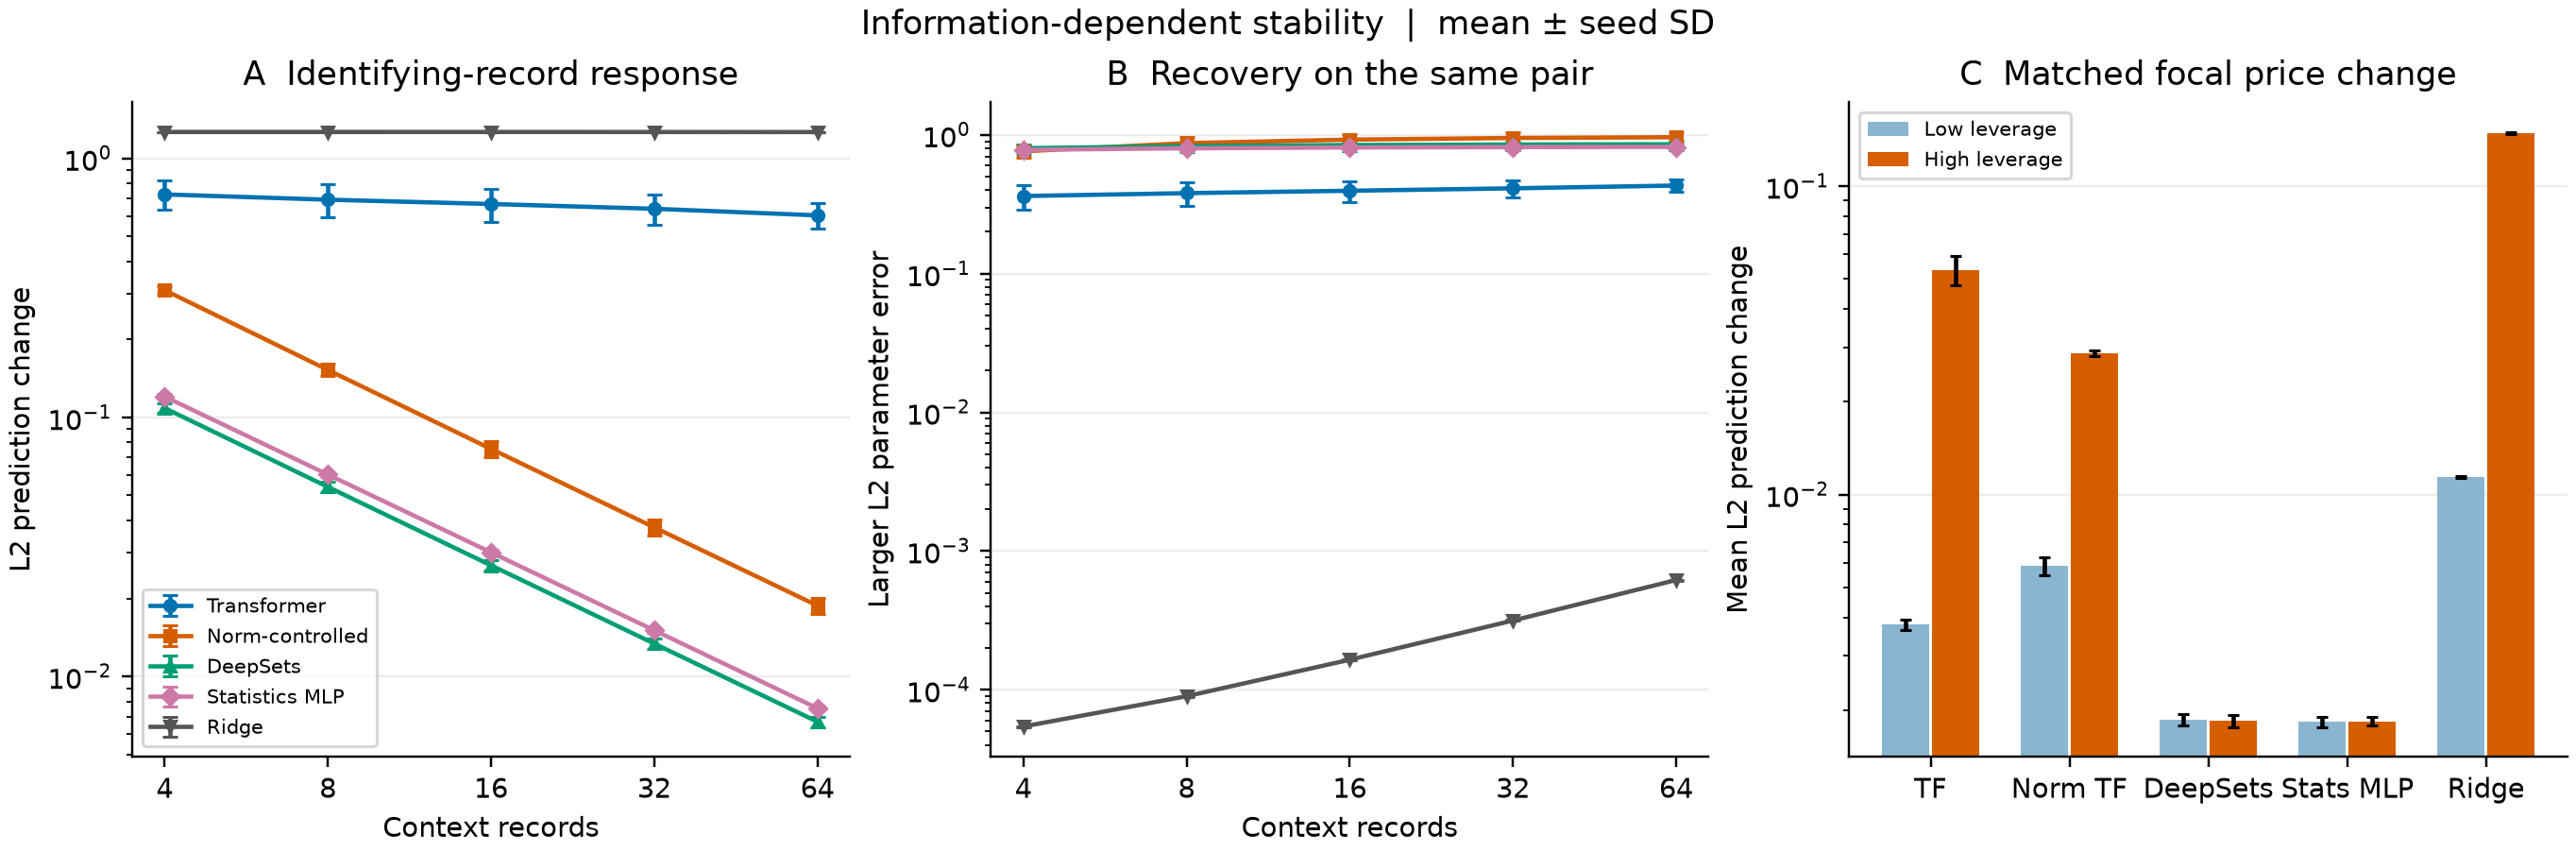
\includegraphics[width=\linewidth]{results/leverage_stability/leverage_stability.png}
\caption{Experiment G. Left and center show the clean cross-task
identifying pair. Right shows the matched, within-task price
perturbation across background designs. Bars denote one standard
deviation across three seed means.}
\label{fig:g}
\end{figure}

\section{Discussion and conclusion}
The lower bound identifies a specific conflict between uniform
stability and uniform accuracy when one record carries a parameter
direction. G shows that the learned response depends on leverage
even at a fixed focal location. Its magnitude and behavior under
clean same-task changes differ from ridge. These are properties of
input-output behavior. Attention weights and perturbation responses
alone leave the internal computation unresolved.

The experiments use two generators, exact dispatch, three seeds,
and mostly noiseless prices. The identifying contexts are deliberate
stress cases, and the architecture's norm-based constant is too loose
to predict a crossover at the tested lengths. The mean replacement
response under a natural sampling distribution remains a separate
quantity. The combination of a worst-case bound, a valid dispatch
construction, and measured leverage responses explains why information
distribution matters when evaluating Transformer stability and recovery.

\clearpage
\begin{thebibliography}{9}
\bibitem{li}
Yingcong Li, Muhammed Emrullah Ildiz, Dimitris Papailiopoulos, and Samet Oymak.
Transformers as algorithms: Generalization and stability in in-context learning.
\emph{ICML}, PMLR 202, pp.\ 19565--19594, 2023.
\href{https://proceedings.mlr.press/v202/li23l.html}{Proceedings}.

\bibitem{keshavarz}
Arezou Keshavarz, Yang Wang, and Stephen Boyd.
Imputing a convex objective function.
\emph{IEEE Multi-Conference on Systems and Control}, pp.\ 613--619, 2011.
\href{https://web.stanford.edu/~boyd/papers/imputed_objective.html}{Author's copy}.

\bibitem{liang}
Zhirui Liang and Yury Dvorkin.
Data-driven inverse optimization for marginal offer price recovery in electricity markets.
\emph{ACM e-Energy}, 2023.
\href{https://arxiv.org/abs/2302.05498}{Preprint}.

\bibitem{akyurek}
Ekin Aky\"urek, Dale Schuurmans, Jacob Andreas, Tengyu Ma, and Denny Zhou.
What learning algorithm is in-context learning? Investigations with linear models.
\emph{ICLR}, 2023.
\href{https://arxiv.org/abs/2211.15661}{Paper}.

\bibitem{deepsets}
Manzil Zaheer, Satwik Kottur, Siamak Ravanbakhsh, Barnab\'as P\'oczos,
Ruslan Salakhutdinov, and Alexander J. Smola.
Deep sets. \emph{NeurIPS}, 2017.
\href{https://papers.nips.cc/paper_files/paper/2017/hash/f22e4747da1aa27e363d86d40ff442fe-Abstract.html}{Proceedings}.

\bibitem{clb}
Abhinav Chakraborty, Yuetian Luo, and Rina Foygel Barber.
Stability and accuracy trade-offs in statistical estimation.
\emph{arXiv:2601.11701}, 2026.
\href{https://arxiv.org/abs/2601.11701}{Preprint}.
\end{thebibliography}

\clearpage
\appendix
\section{Proof of Theorem~\ref{thm:upper}}
\label{app:encoder}
For row states \(h_i,h_i'\) at one layer input write
\(e_i=\norm{h_i-h_i'}\) and \(\bar e=m^{-1}\sum_i e_i\).
All state norms have a common bound at each fixed layer, independent
of \(m\). The embedding maps bounded inputs to bounded states.
Attention returns a convex combination of bounded values in each
head. The subsequent finite affine maps, residuals, and rowwise
nonlinearities preserve boundedness. In particular, centering and
normalizing a width-\(p\) row before its LayerNorm affine map gives
a vector of norm at most \(\sqrt p\).

For a head of dimension \(d_h\), let \(Q_0,K_0,V_0\) bound the norms
of its query, key and value vectors, including affine biases, and
write \(q,k,v\) for the operator norms of the corresponding linear
maps. Its score in row \(i\), column \(j\), is
\(s_{ij}=q_i^\top k_j/\sqrt{d_h}\). For the two input matrices we have
\[
 |s_{ij}|,|s'_{ij}|\le B=Q_0K_0/\sqrt{d_h},
 \qquad |s_{ij}-s'_{ij}|\le
 (qK_0e_i+kQ_0e_j)/\sqrt{d_h}.
\]
The latter follows by adding and subtracting the inner product of
the new query with the old key. On the line segment between the two
score rows, every softmax entry is at most \(e^{2B}/m\), since the
numerator is at most \(e^B\) and the denominator at least \(me^{-B}\).
For \(p=\softmax(s)\), the \(j\)-th column of its Jacobian has absolute
sum \(2p_j(1-p_j)\le2p_j\). Integrating this Jacobian along the segment
gives
\[
 \lVert p_i-p_i'\rVert_1
 \le \frac{2e^{2B}}{\sqrt{d_h}}(qK_0 e_i+kQ_0\bar e).
\]
For the head output, changing weights with values fixed costs at
most \(V_0\lVert p_i-p_i'\rVert_1\). Changing values with weights fixed
costs at most \(ve^{2B}\bar e\). Averaging over rows bounds the mean
head difference by \(J_h\bar e\), where
\[
 J_h=e^{2B}\left(v+\frac{2V_0(qK_0+kQ_0)}{\sqrt{d_h}}\right).
\]
Concatenation bounds its mean difference by the sum of the individual
head bounds. Applying \(W_O\) and adding the input residual gives a
factor at most \(1+\|W_O\|\sum_hJ_h\). Here and below, matrix norms
are induced Euclidean operator norms.

To bound LayerNorm, write \(P\) for the orthogonal projection onto
mean-zero rows. The map before its learned affine part is
\(h\mapsto Ph/(\|Ph\|_2^2/p+\eta)^{1/2}\), with \(\eta>0\).
The derivative of \(z\mapsto z/(\|z\|_2^2/p+\eta)^{1/2}\)
has tangential eigenvalue \((\|z\|_2^2/p+\eta)^{-1/2}\) and radial
eigenvalue \(\eta(\|z\|_2^2/p+\eta)^{-3/2}\). Each is at most
\(1/\sqrt\eta\). Consequently a LayerNorm with learned gain \(\gamma\)
has Lipschitz constant at most \(\|\gamma\|_\infty/\sqrt\eta\).
The two affine feedforward maps and ReLU, with their residual,
contribute another factor at most \(1+\|W_2\|\|W_1\|\).
Each of the two LayerNorm maps and both residual blocks therefore
have a finite layer product. This covers the implemented post-residual
block, with actual attention scores scaled by \(1/\sqrt{16}\).

Initially just one row differs and its embedded difference is at most
\(2R_{\rm in}\|W_{\rm emb}\|\), where \(R_{\rm in}\) bounds the record
feature norm. Thus \(\bar e_0\le 2R_{\rm in}\|W_{\rm emb}\|/m\).
The finite product of layer factors propagates this bound. The difference
of mean-pooled vectors is at most the final \(\bar e\) by the triangle
inequality. The sigmoid affine-box readout multiplies the bound by at
most \(\|\diag(\mathrm{span})\|\|W_{\rm head}\|/4\). This proves the
claim. The box gives a separate trivial bound on all outputs. For the
three uncapped checkpoints the norm substitution gave
\(\log_{10} C\) between 616.5 and 708.9, so the box is tighter over
the measured lengths.

\section{Supporting task-level transfer bound}
\label{app:transfer}
Let \(m\) be fixed and \(L_\theta(f)\) be the conditional expectation
of span-normalized squared parameter error over contexts from task
\(\theta\). Both estimates and targets are in the coefficient box,
so \(L_\theta(f)\in[0,1]\). Take \(T\) independent source tasks from
a population \(P\), and a fixed hypothesis class independent of those
tasks. For a finite \(\varepsilon\)-cover of the induced task-risk
functions in sup norm with size \(N_\varepsilon\), with probability
at least \(1-\delta\) all predictors in that class satisfy
\[
 \left|\mathbb E_{\theta\sim P}L_\theta(f)
   -\frac{1}{T}\sum_{t=1}^T L_{\theta_t}(f)\right|
 \le 2\varepsilon+\sqrt{\frac{\log(2N_\varepsilon/\delta)}{2T}} .
\]
For each center Hoeffding's inequality gives a two-sided tail
\(2e^{-2Tu^2}\) at deviation \(u\). A union bound controls every
center, and approximation of the population and empirical risks
costs \(\varepsilon\) each. At fixed \(m\), a deterministic compact
weight set gives a finite cover via uniform continuity of the
network and its bounded loss on the bounded record domain.
This argument controls the source-to-population risk difference
for that class. The numerical size of the cover, optimization
quality, and transfer under a different task distribution require
other information. The assumption of independent source tasks and
fresh evaluation contexts matches the in-distribution target
comparison in E. The bound makes no empirical rate prediction for
the optimization-budget sweep.

\section{Result provenance}
\label{app:results}
\begingroup
\raggedright
The paper consolidates saved experiments. Table~\ref{tab:d} uses
the stability and recovery summaries in
\texttt{results/transformer\_stability}. Table~\ref{tab:e} uses
the risk summary in \texttt{results/task\_scaling} at \(m=32\).
Table~\ref{tab:f} uses the context summary in
\texttt{results/context\_informativeness}. Figure~\ref{fig:g}
and the leverage results use the paired-context and intervention
summaries in \texttt{results/leverage\_stability}. The controlled
replications use the identification and matched transfer summaries
in \texttt{results/leverage\_followup}. The report's input figure is
included as an existing repository asset. The unit-test command is
\texttt{python -m unittest discover -s tests -v}.\par
\endgroup
\end{document}
